\chapter{Review of Fundamentals}

\section{Complex Number Concepts required for EE233}\label{cnconcepts}
\begin{itemize}
  \item $j = \sqrt{-1}$
  \item complex number is the sum of a real part, $\sigma$ + an imaginary part $j\omega$ (where $\omega$ is a real number to be multiplied by $j$.)
  \item   The {\it magnitude} of a complex number is the Pythagorean sum of the real and imaginary parts:
  If $x= a+jb$ is a complex number, then the magnitude is
  \[
  |x| = \sqrt{a^2+b^2}
  \]
  \item To add together two complex numbers, add their real and imaginary parts separately.
  \[
  x = a+bj \qquad y = c+dj
  \]
  \[
  x + y = (a+c) + j(b+d)
  \]
  \item To multiply two complex numbers, multiply them together like two first order polynomials in $j$ (using the definitions above)
  \[
  x*y = (a+bj)*(c+dj) = ac+adj + bcj+bdj^2
  \]
  since $j^2=-1$ we have
  \[
  x*y = (ac-bd)+(ad+bc)j
  \]

  \item Complex numbers describe a point in the {\it complex plane}.  The $X$ axis of the complex plain is the real part of the complex number and the $Y$ axis is the imaginary part.

  \item To plot the point $a+jb$ on the complex plane, plot a point at $X = a, \: Y = b$.

  \item The magnitude of a complex number is the distance from the origin to its point on the complex plane.

  \item The {\it angle} of a complex number is the angle formed from the positive real axis ($X>0$) and the line between the origin and the point.

  \item There is an \href{http://en.wikipedia.org/wiki/Euler\%27s_formula}{exponential form} of any complex number:
  \[
  e^{j\theta} = \cos(\theta) + j\sin(\theta)
  \]
  \item To convert a complex number to exponential form we invert the previous equation:
  \[
  a+bj = |a+bj| e^{j\tan^{-1}(b/a)}
  \]

  \item The $\tan^{-1}()$ function traditionally limits us to quadrants I and IV of the complex plain.    More generally we can use the 4-quadrant 2-argument arctan function \href{http://en.wikipedia.org/wiki/Atan2}{({\tt atan2(b,a)}) }.

  \item A consequence of multiplication of complex numbers and the exponential represenation of complex numbers is that when we multiply two complex numbers:
     \begin{quotation} {\it ``angles add and magnitudes multiply''}
     \end{quotation}
   if $A,B,C$ are complex numbers and $C = A * B$
   \[
    \angle{C} = \angle{A}+\angle{B}  \qquad   |C| = |A|*|B|
   \]


\end{itemize}

\subsubsection{Kahn Academy Videos}\label{KahnV}

\href{https://www.khanacademy.org/math/algebra/complex-numbers/complex_numbers/v/complex-numbers}{complex numbers}

\href{https://www.khanacademy.org/math/trigonometry/imaginary_complex_precalc/complex_analysis/v/exponential-form-to-find-complex-roots}{exponential form of complex numbers}




\newpage
\section{Complex Numbers}


Complex numbers make use of the famous imaginary number
$i = \sqrt{-1}$.    In ECE that is confusing with current so we use instead
\[
  j = \sqrt{-1}
\]

An {\it imaginary} number is any real number multiplied by $j$ such as
\[
10j,\; -4j,\; 14.7j, \; \mathrm{etc.}
\]

A {\it complex} number is the sum of a real number plus an imaginary number:
\[
  Z = a + bj
\]

\subsection{Complex Plane}

We represent complex numbers in the {\it Complex Plane}.   The complex plane is
a version of the $X,Y$ plane where each complex number represents a point or vector.
The real part is the $X$ coordinate and the imaginary part is the $Y$ coordinate.

For example the two complex numbers

\[
Z_1 = 2 + 3j, \quad Z_2=-1-3j
\]
can be drawn on the complex plane below as:

[Graphic]
\vspace{3.5in}
%\includegraphics[width=0.5\textwidth]{figsChapt01/MR6732.png}

Like any plane, the complex plane can also be addressed in polar coordinate form.
Below is the relationship between the complex number components in Cartesian and
polar forms:

\vspace{0.15in}
\begin{align}
\text{Complex} &    & \text{Polar}  \\ \hline
Z &= a + bj & &= r\angle\theta \\
a &= \text{Re}\{Z\} & r &= \sqrt{a^2+b^2} & \text{Magnitude} \\
b &= \text{Im}\{Z\} & \theta &= \tan^{-1}\left(\frac{b}{a}\right) & \text{Angle}
\end{align}


\subsection{Exponential Form}

One of the most famous equations in mathematics is Euler's Identity:
\begin{equation}
\boxed{e^{j\theta} = \cos(\theta) + j\sin(\theta)}
\end{equation}

\begin{equation}
e^{j\pi} = -1
\end{equation}



\subsection{ Computation with Complex Numbers}

\noindent Rectangular Form:
\[
\text{Addition:}       \quad  (a + bj) + (c + dj) = (a+c) + (b+d)j
\]
\[
\text{Multiplication:} \quad  (a + bj) \times (c + dj) = ac + adj + bcj + bdj^2 = ac-bd + (ad+bc)j
\]

\noindent Polar Form:

\[
\text{Addition:} \quad       r_1\angle\theta_1 + r_2\angle\theta_2
\]
\[
\text{Multiplication:} \quad (r_1\angle\theta_1)\times(r_2\angle\theta_2 = r_1r_2\angle(\theta_1+\theta_2)
\]

So each operation (addition or Multiplication) is easiest in one of the two forms, summed up with the slogan
\begin{quotation}``Angles add, Magnitudes multiply''\end{quotation}

\noindent{Exponential Form}
Note that the polar form is derived from Euler's exponential form:
\begin{align}
\text{Addition:} \quad &\text{Euler's $e^{j\alpha}$} \\
\text{Multiply:} \quad &A_1e^{j\theta_1} \cdot A_2e^{j\theta_2} = A_1A_2e^{j(\theta_1+\theta_2)}
\end{align}



\subsection{Complex Conjugate}
If $Z = a + jb$ then its complex conjugate, $Z^* = a - jb $, in other words to get the Complex conjugate of  a complex
number, just multiply its imaginary part by $-1$.
If we multiply a complex number by its conjugate, it is easy to see that we get its Magnitude:

\[
ZZ^* =  (a+bj)(a-bj) = a^2 - abj + abj - b^2j^2 = a^2 + b^2
\]

[Graphic]
%\includegraphics[width=0.5\textwidth]{figsChapt01/MR6733.png}


\begin{align}
\text{e.g. Division:} \quad \frac{Z_1}{Z_2} &= \frac{a_1 + b_1j}{a_2 + b_2j} = \frac{Z_1 \cdot Z_2^*}{Z_2 \cdot Z_2^*} = \frac{Z_1Z_2^*}{|Z_2|^2}
\end{align}

\subsection*{Complex Number Arithmetic in a nutshell:}
\begin{tabular}{l|p{1.in}|p{1.0in}|p{1.0in}}
Form                 & Add           & Multiply           & Conjugate \\\hline
Rectangular, $a+bj$  & By Component  & Like a Polynomial  & Negate imaginary part\\ \hline
Polar,
$A\angle{\theta}$    & like Vectors  & Angles Add, Magnitudes Multiply & Negate Angle \\ \hline
Exponential,
$Ae^{j\theta}$       & Convert to rectangular! & just like Polar & Negate exponent
\end{tabular}

\subsection{Examples}

Q: What is $\sqrt{-64}$?

A: $\sqrt{-1 \cdot 64} = \sqrt{-1} \cdot 8 = j8$ or imaginary \#

Q: What is $2 + \sqrt{-36}$?


A: $2 + j6$, which can't be simplified, the solution is
a Complex \# that can be considered to
be two projections of a  vector.

We think of $j$ as a unit vector $90^\circ$ away from the real axis.


Therefore, their sum is the projection of their vector
sum:
\subsection{Magnitude}
$r = \sqrt{2^2 + 6^2} = \sqrt{4 + 36} = 6.32$
\subsection{Angle}
$\theta = \tan^{-1}\left(\frac{36}{4}\right) = 83.66^\circ = 1.46 \text{ rad}$

\subsection{two Complex numbers}

\[
A = 3+5j,\; B = -2-2j
\]

(the easy way):
\[
A+B = (3-2) + (5-2)j = 1+3j
\]

\subsection{the hard way }
Consider them as magnitude/angle:
\[
|A| = \sqrt{3^2+5^2} = 5.83,\; \angle{A} = \tan^{-1}(5/3) = 71.5^\circ
\]
\[
|B| = \sqrt{2^2+2^2} = 2.83,\; \angle{B} = \mathrm{atan2}(-2,-2) = 225^\circ
\]
(note can't use $\tan^{-1}$!)
Now adding is like vectors:


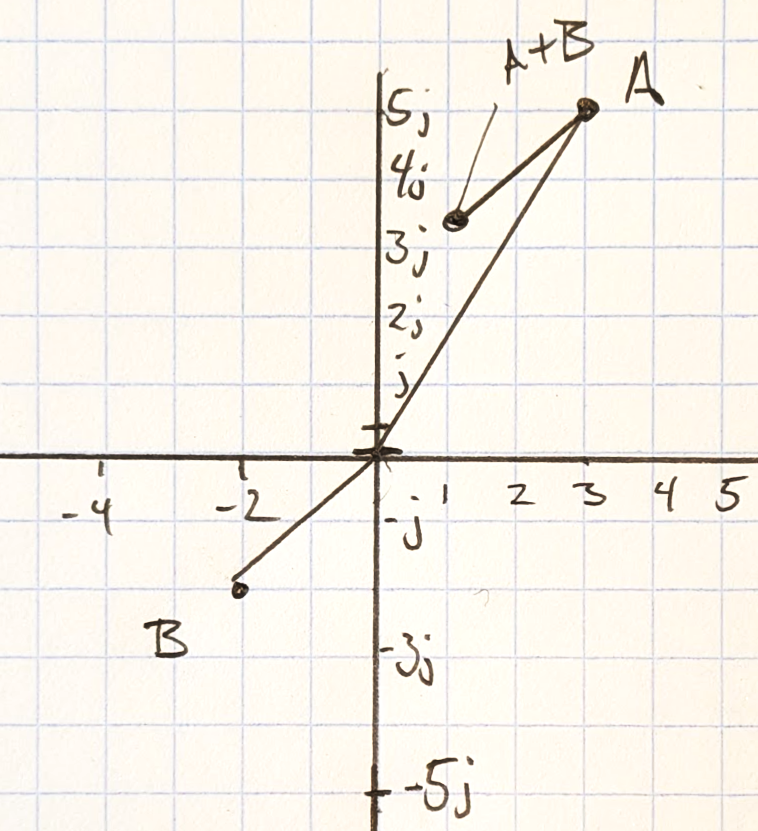
\includegraphics[width=.5\textwidth]{figsChapt01/AA65506.png}







\section{Kirchoff's Current and Voltage Laws (KCL, KVL)}

\subsection{KCL}
In our context we can express KCL as follows:

If a node connects $n$ conductors having currents, $i_1 \dots i_n$,
then
\[
\sum_k i_k = 0
\]
Physically this means that charge cannot accumulate on a node and give it a
potential (of course a capacitor {\it can} accumulate charge!).

\subsection{KVL}
Our version of KVL states:

If a circuit loop, consists of $n$ nodes (which may belong to other loops as well),
and we define the $k^{th}$ branch as the branch connecting node $k$ with node $k-1$, and if $V_k$ is defined as the voltage drop across the branch:
\[
V_k = v_k - v_{k-1}
\]
(where $v_k$ is the voltage at node $k$)
then KVL is
\[
\sum_k V_k = 0
\]
In words, the sum of the voltage drops around any loop is equal to zero. In an
every day example, if you walk any closed path around the streets of Seattle,
your net gain in elevation (net change of potential energy) must be zero.

For more complex circuits having more than one node or loop,
KCL and KVL are frequently used to generate a set of equations which can be
jointly solved to get all the node voltages or branch currents.


\subsection{KCL/KVL examples}


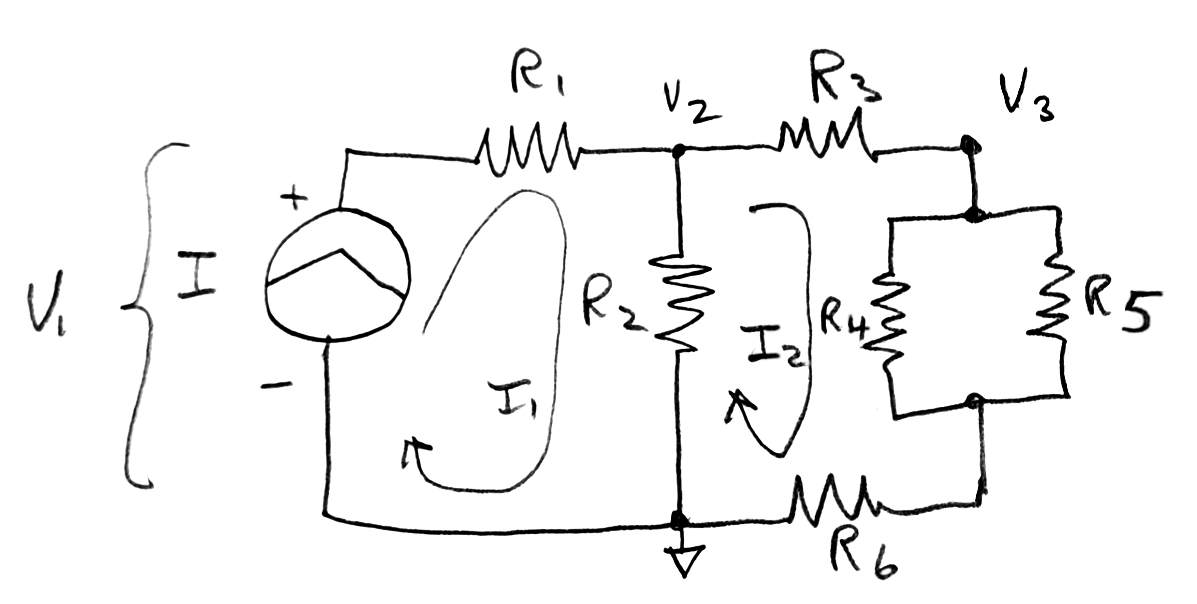
\includegraphics[width=.75\textwidth]{figsChapt01/IG95777.png}

\subsection{KVL}
 Write two KVL equations for the two loops above (|| resistors don't count as a loop!).

1)
\[
V_1+I_1R_1+(I_1+I_2)R2=0
\]

2)
\[
I_2R_3+I_2(R_4||R_5)+I_2R+6+(I_2-I_1)R_2=0
\]

\subsection{KCL}
For the same circuit, write a KCL equation for the node which joins $R_1,R_2,R_3$,  in terms
of the three node voltages:
\[
\frac{V_1-V_2}{R_1}+\frac{-V_2}{R_2} + \frac{V_3-V_2}{R_3} = 0
\]


\section{Basic Operational Amplifier Configurations}


\subsection{Inverting Amplifier}

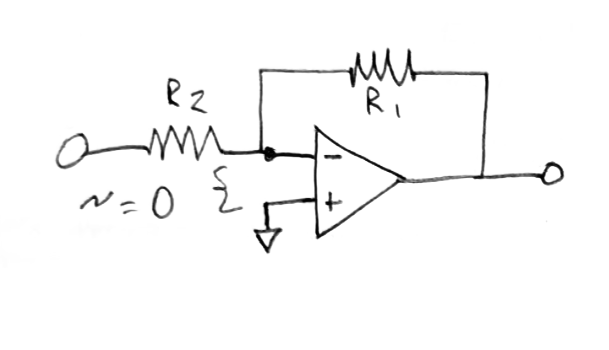
\includegraphics[width=60mm]{figsChapt01/BV83562.png}


\[
G = \frac {-R1}  {R2}
\]
\subsection{Non-inverting Amplifier}
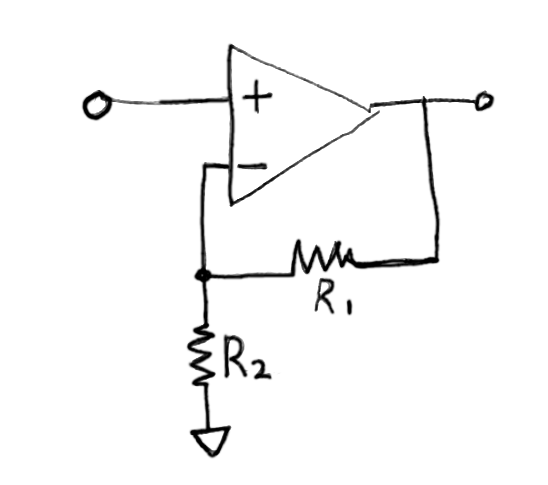
\includegraphics[width=50mm]{figsChapt01/PN49388.png}
\[
G=\frac {+R1}  {R1+R2}
\]
\subsection{Summing Amplifier}
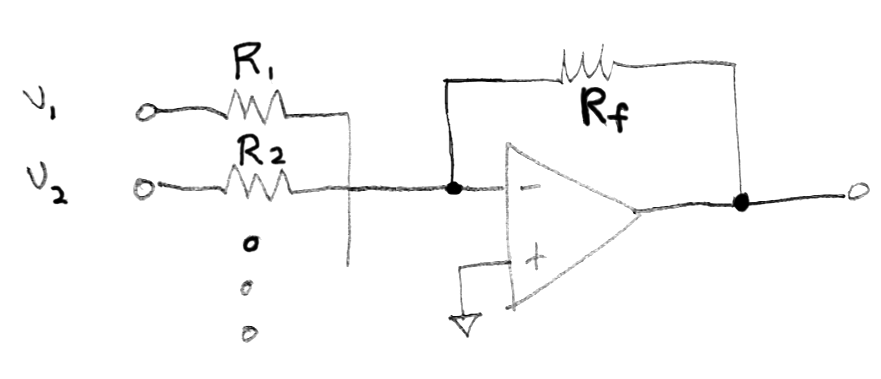
\includegraphics[width=90mm]{figsChapt01/GC91051.png}
\[
V_O= -V_i\sum_i \frac {R_f}  {R_i}
\]
\subsection{Voltage Follower}
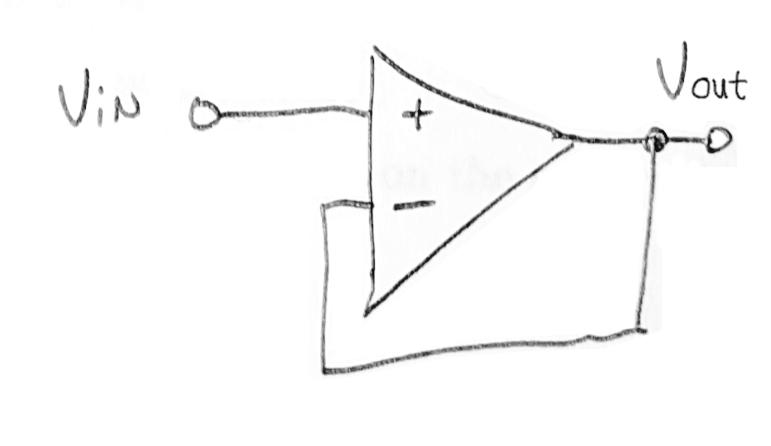
\includegraphics[width=50mm]{figsChapt01/BI19090.png}
\[
V_O = V_{in}
\]
\section{deciBells (dB)}


\subsection{Decibels}

Decibels are a logarithmic\footnote{Take the quiz and review logs if necessary: Section \ref{LogReview}} unit which are widely used for the analysis of frequency response.   If we have a quantity, $x$, then
\[
dB(x) = 20\log_{10}(x)
\]
where $dB(x)$ represents the decibel representation of $x$.


Because decibels are logarithmic units, we will make frequent use of the following properties (which are easily proved using basic properties of logarithms)

\[
dB(ab) = dB(a)+ dB(b)
\]
\[
dB(a/b) = dB(a) - dB(b)
\]
\[
dB(\sqrt{a}) = \frac {dB(a)}{2}
\]
etc.

Some handy {\it approximate} $dB$ values, when  memorized, give you very quick and accurate (within 5\%) hand calculation results:

\[
3.16 = \sqrt{10} = 10dB ,\quad 10 = 20dB, \quad 100 = 40dB
\]
\[
2 = 6dB, \quad   \sqrt{2} = 3dB
\]
\[
1/2 = -6dB, \quad \frac{1}{\sqrt{2}} = \frac{\sqrt{2}}{2} = -3dB
\]
etc.


\begin{ExampleSmall}
Convert the following quantities to $dB$.

\[
dB(1000) = 20\log(1000) = 20*3 = 60dB
\]
\[
dB(6000) = dB(1000\times6) = dB(1000) + dB(6)  = 60 + 15.6 = 76.6dB
\]
\[
dB(X/100) \quad (\mathrm{where }\quad dB(X)=40dB) = 40 - 20\log(100) = 40-40 = 0dB
\]

\end{ExampleSmall}

\section{2, and 4 quadrant arc-tangent functions}

It's easy to see that
regular arctangent is limited to quadrants I and IV!

\vspace{2.5in}
\[
tan^{-1}(\frac {-5}  {-3} ) = tan^{-1}(\frac {5}  {3} )
\]


The real word goes around the
whole circle, so we define the 4-quadrant arctan function:
\[
\mathrm{atan2}(Y,X)
\]
which figures out the right way to apply arctan() depending on the quadrants.


\section{Voltage Dividers}


\section{Series and Parallel Resistors}


\vspace{3.0in}
\section{Thevenin and Norton equivalent circuits}

\subsection{Thevenin}
\vspace{3.5in}
Thevenin Stuff

\subsection{Norton}
\vspace{3.5in}
Norton Stuff


\section{Energy Storage Elements}

\subsection{Capacitors}

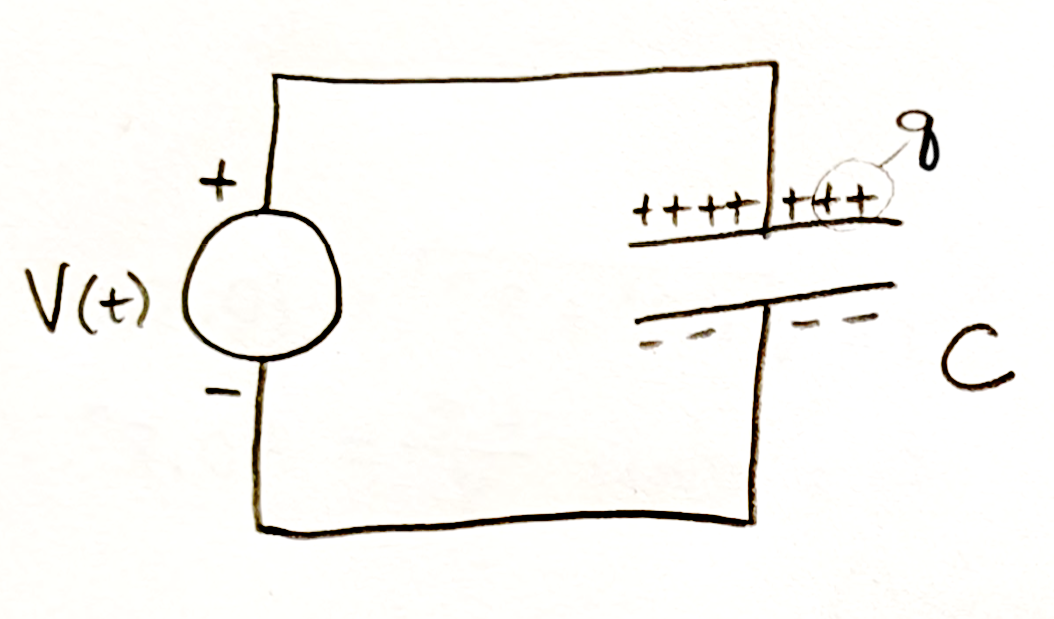
\includegraphics[width=.5\textwidth]{figsChapt01/SA77254.png}

Charge:
\[
q = CV
\]
Current
\[
i = \frac {dq}  {dt}  = C\frac {dV}  {dt}
\]
Charge
\[
q = \int_{-\infty}^t i dt =  \int_{-\infty}^t  C\frac {dV}  {dt}
\]
Voltage
\[
V = 1/C \int_{0}^t i dt+ \int_{-\infty}^0 i dt + 1/C q_{(t=0)}
\]
\[\boxed{
V=\frac {1}  {C} \int_{-\infty}^t i\; dt }
\]

Energy
\[
E_C = \int_{-\infty}^t V(t)i(t)dt = \int_{-\infty}^t VC\frac {dV}  {dt} = C\int_{-\infty}^t VdV
\]
\[
= \left . \frac {1}  {2}CV^2(t)\right | ^t_{-\infty} \;\;
\]
Finally
\[
E_C(t) = \frac {1}  {2}CV^2(t) \; \mathrm{, assume~ } V(-\infty) = 0 \;\mathrm(Joules)
\]

\subsection{Inductors}

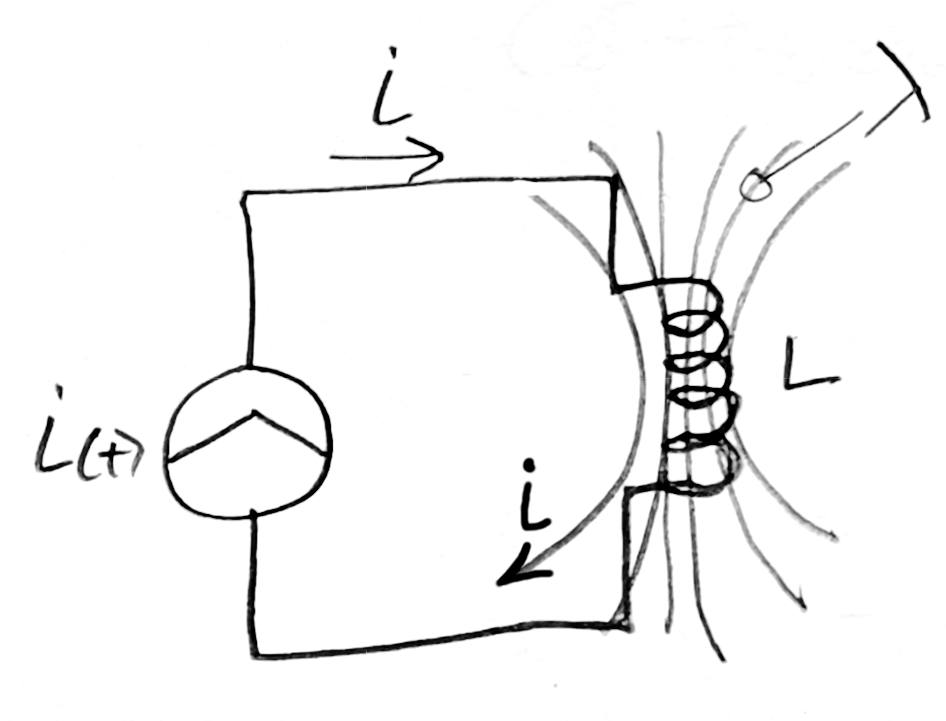
\includegraphics[width=.5\textwidth]{figsChapt01/GM98526.png}

Mag Field:
\[
\lambda = Li
\]
Voltage
\[
V = \frac {d\lambda}  {dt} = \frac {d}  {dt} Li
\]
\[\boxed{
V(t) =  L\frac {di}  {dt}   }
\]
Energy
\[
E_L = \int_{-\infty}^t V i\; dt = \int_{-\infty}^t L\frac {di}  {dt} i \;dt
\]
\[
L\int_{-\infty}^t i\; di = \frac {1}  {2} Li^2(t)  \; \mathrm{(Joules)}
\]


